%% -*- coding: utf-8 -*-
\documentclass[12pt,a4paper]{scrartcl} 
\usepackage[utf8]{inputenc}
\usepackage[english,russian]{babel}
\usepackage{indentfirst}
\usepackage{misccorr}
\usepackage{graphicx}
\usepackage{amsmath}
\usepackage{float}

\usepackage{xcolor}
\usepackage{hyperref}
\hypersetup{colorlinks,
  pdftitle={The title of your document},
  pdfauthor={Your name},
  allcolors=[RGB]{000 000 000}}

\begin{document}
\begin{titlepage}
  \begin{center}

    Санкт-Петербургский политехнический университет Петра Великого

    \vspace{0.25cm}
    
    Институт прикладной математики и механики
    
    Кафедра «Прикладная математика»
    \vfill

	\vspace{0.25cm}
	    Отчёт\\
	по лабораторной работе №1\\
	по дисциплине\\
	«Математическая статистика»

  \bigskip

\end{center}
\vfill

\newlength{\ML}
\settowidth{\ML}{«\underline{\hspace{0.7cm}}» \underline{\hspace{2cm}}}
\hfill\begin{minipage}{0.4\textwidth}
  Выполнил студент\\ В.\,А.~Рыженко\\
\end{minipage}%
\bigskip

\hfill\begin{minipage}{0.4\textwidth}
  Проверил:\\
к.ф.-м.н., доцент\\
Баженов Александр Николаевич\\
\end{minipage}%
\vfill

\begin{center}
  Санкт-Петербург, 2020 г.
\end{center}
\end{titlepage}

\tableofcontents
\listoffigures
\newpage

\section{Постановка задачи}
 
Для 5 распределений:
\begin{itemize}
 \item Нормальное распределение N(x, 0, 1)
 \item Распределение Коши C(x, 0, 1)
 \item Распределение Лапласа L(x, 0, $\frac{1}{\sqrt2}$)
 \item Постановка задач исследованияРаспределение Пуассона P(k, 10)
 \item Равномерное распределение U(x, $-\sqrt{3}, \sqrt{3}$) 
\end{itemize}

\begin{enumerate}
 \item Сгенерировать выборки размером 10, 50 и 1000 элементов.
Построить на одном рисунке гистограмму и график плотности распределения.

\item Сгенерировать выборки размером 10, 100 и 1000 элементов.
Для каждой выборки вычислить следующие статистические характеристики положения данных:
$\overline x ~\eqref{eq:mean}, med\, x~\eqref{eq:med}, z_R ~\eqref{eq:semisum}, z_Q ~\eqref{eq:semiquartile}, z_tr~\eqref{eq:trim}$. Повторить такие
вычисления 1000 раз для каждой выборки и найти среднее характеристик положения и их квадратов:\begin{equation}\label{eq:expectation}
\centering
 E(z) = \overline z
\end{equation}

Вычислить оценку дисперсии по формуле:

\begin{equation}\label{eq:dispertion}
\centering
 D(z) = \overline {z^2} - \overline z^2
\end{equation}

Представить полученные данные в виде таблиц.

\item

Сгенерировать выборки размером 20 и 100 элементов.
Построить для них боксплот Тьюки.
Для каждого распределения определить долю выбросов экспериментально (сгенерировав выборку, соответствующую распределению 1000
раз, и вычислив среднюю долю выбросов) и сравнить с результатами,
полученными теоретически.

\item

Сгенерировать выборки размером 20, 60 и 100 элементов.
Построить на них эмпирические функции распределения и ядерные
оценки плотности распределения на отрезке [-4; 4] для непрерывных
распределений и на отрезке [6; 14] для распределения Пуассона.

\end{enumerate}
 
\section{Теория}

\subsection{Распределения}

\begin{itemize}
\begin{item}
Нормальное распределение
\begin{equation}\label{eq:Normal}
\centering
 N(x, 0, 1) = \frac{1}{\sqrt{2\pi} } e^{-\frac{x^2}2}
\end{equation}
\end{item}

\begin{item}
Распределение Коши
\begin{equation}\label{eq:Cauchy}
\centering
 C(x, 0, 1) = \frac{1}{\pi} \frac{1}{x^2 + 1}
\end{equation}
\end{item}

\begin{item}
Распределение Лапласа
\begin{equation}\label{eq:Laplace}
\centering
L(x, 0, \frac{1}{\sqrt2}) = \frac{1}{\sqrt{2} } e^{\sqrt2|x|}
\end{equation}
\end{item}

\begin{item}
Распределение Пуассона
\begin{equation}\label{eq:Poisson}
\centering
P(k, 10) = \frac{10^k}{k! } e^{-10}
\end{equation}
\end{item}

\begin{item}
Равномерное распределение
\begin{equation}\label{eq:Uniform}
\centering
U(x, -\sqrt{3}, \sqrt{3})  = 
\begin{cases}
\frac{1}{2\sqrt3}, &\mbox{при } |x| \leq \sqrt3 \\ 0 , &\mbox{при } |x| \textgreater \sqrt3
\end{cases}
\end{equation}
\end{item}
\end{itemize}

\subsection{Характеристики положения}

\begin{itemize}
\begin{item}
Выборочное среднее
\begin{equation}\label{eq:mean}
\centering
\overline x =\frac{1}{n}\sum_{i=1}^n x_i
\end{equation}
\end{item}

\begin{item}
Выборочная медиана
\begin{equation}\label{eq:med}
\centering
med x =
\begin{cases}
x_{(l + 1)} &\mbox{при  $n = 2l + 1$} \\ \frac{x_{(l)} + x_{(l + 1)}}{2} &\mbox{при  $n = 2l$}
\end{cases}
\end{equation}
\end{item}

\begin{item}
Полусумма экстремальных выборочных элементов
\begin{equation}\label{eq:semisum}
\centering
z_R = \frac{x_{(1)} + x_{(n)}}{2}
\end{equation}
\end{item}

\begin{item}
Полусумма квартилей \\
Выборочная квартиль $z_p$ порядка $p$ определяется формулой
\begin{equation}\label{eq:quartile}
\centering
z_p =
\begin{cases}
x_{([np] + 1)} &\mbox{при  $np$ дробном} \\ x_{(np)} &\mbox{при  $np$ целом}
\end{cases}
\end{equation}
Полусумма квартилей
\begin{equation}\label{eq:semiquartile}
\centering
z_Q = \frac{z_{1/4} + z_{3/4}}{2}
\end{equation}

\end{item}

\begin{item}
Усечённое среднее
\begin{equation}\label{eq:trim}
\centering
z_R = \frac{1}{n - 2r} \sum_{i=r+1}^{n - r} x_{(i)}, r \approx \frac{n}{4}
\end{equation}
\end{item}

\end{itemize}

\subsection{Характеристики рассеяния}
Выборочная дисперсия

\begin{equation}\label{eq:samplevariance}
\centering
D = \frac{1}{n} \sum_{i=1}^{n} x_i - \overline x
\end{equation}

\subsection{Боксплот Тьюки}
\subsubsection{Определение}

Боксплот (англ. box plot) — график, использующийся в описательной статистике, компактно изображающий одномерное распределение вероятностей.

\subsubsection{Описание}

Такой вид диаграммы в удобной форме показывает медиану, нижний и верхний квартили и выбросы. Несколько таких ящиков можно нарисовать бок
о бок, чтобы визуально сравнивать одно распределение с другим; их можно располагать как горизонтально, так и вертикально. Расстояния между
различными частями ящика позволяют определить степень разброса (дисперсии) и асимметрии данных и выявить выбросы.

\subsubsection{Построение}

Границами ящика служат первый и третий квартили, линия в середине
ящика — медиана. Концы усов — края статистически значимой выборки
(без выбросов). Длину «усов» определяют разность первого квартиля и полутора межквартильных расстояний и сумма третьего квартиля и полутора
межквартильных расстояний. Формула имеет вид

\begin{equation}\label{eq:borders}
\centering
X_1 = Q_1 - \frac{3}{2}(Q_3 - Q_1), X_2 = Q_3 + \frac{3}{2}(Q_3 - Q_1),
\end{equation}

где $X_1$ — нижняя граница уса, $X_2$ — верхняя граница уса, $Q_1$ — первый
квартиль, $Q_3$ — третий квартиль.
Данные, выходящие за границы усов (выбросы), отображаются на графике
в виде маленьких кружков

\subsection{Теоретическая вероятность выбросов}

По формуле ~\eqref{eq:borders}можно вычислить теоретические нижнюю и верхнюю границы уса
($X_1^T$ и $X_2^T$ соответственно).
Выбросами считаются величины $x$, такие что:
\begin{equation}\label{eq:emissions}
\centering
\left[ 
      \begin{gathered} 
       x \textless X_1^T \\
	  x \leq X_2^T \\
      \end{gathered} 
\right.
\end{equation}

Теоретическая вероятность выбросов для непрерывных распределений

\begin{equation}\label{eq:prob1}
\centering
P_B^T = P(x < X_1^T) + P(X > X_2^T) = F(X_1^T) + (1 - F(X_2^T)),
\end{equation}

где $F(X) = P(x\textgreater X) $ - функция распределения. \\

Теоретическая вероятность выбросов для дискретных распределений
\begin{equation}\label{eq:prob2}
\centering
P_B^T = P(x < X_1^T) + P(X > X_2^T) = (F(X_1^T) - P(x = X_1^T)) + (1 - F(X_2^T)),
\end{equation}

где $F(X) = P(x\textgreater X) $ - функция распределения.

\subsection{Эмпирическая функция распределения}
\subsubsection{Определение}

Эмпирической (выборочной) функцией распределения (э. ф. р.) называется
относительная частота события $X < x$, полученная по данной выборке:

\begin{equation}\label{eq:EmpDistr}
\centering
F_n^*(x) = P^*(X < x).
\end{equation}

\subsubsection{Описание}

Для получения относительной частоты $P^*(X < x)$ просуммируем в статистическом ряде, построенном по данной выборке, все частоты $n_i$, для которых элементы $z_i$ статистического ряда меньше $x$. Тогда $P^*(X < x) = \frac{1}{n}\sum_{z_i < x} n_i.$

\subsection{Оценки плотности вероятности}
\subsubsection{Определение}

Оценкой плотности вероятности $f(x)$ называется функция $\hat{f}(x)$, построенная на основе выборки, приближённо равная $f(x)$

\subsubsection{Ядерные оценки}

Представим оценку в виде суммы с числом слагаемых, равным объёму выборки:

\begin{equation}\label{eq:KernelEstimate}
\centering
\hat{f}_n(x) = \frac{1}{nh_n}\sum_{i=1}^n K(\frac{x-x_i}{h_n}).
\end{equation}

Здесь функция $K(u)$, называемая ядерной (ядром), непрерывна и является
плотностью вероятности, $x_1, ... , x_n$ — элементы выборки, {$h_n$} — любая
последовательность положительных чисел, обладающая свойствами

\begin{equation}
\centering
h_n \underset{n \to \infty}{\longrightarrow} 0;  \, \frac{h_n}{n^{-1}} \underset{n \to \infty}{\longrightarrow} \infty;
\end{equation}

Гауссово (нормальное) ядро

\begin{equation}
\centering
K(u) = \frac{1}{\sqrt{2\pi} } e^{-\frac{u^2}2}
\end{equation}

Правило Сильвермана

\begin{equation}
\centering
h_n = 1.06\hat{\sigma}n^{-1/5},
\end{equation}

где $\hat{\sigma}$ - выборочное стандартное отклонение.

\section {Реализация}
Лабораторная работа выполнена с помощью встроенных средств языка программирования Python в среде разработки Jupyter Notebook и Visual Code. Исходный код лабораторной
работы приведён в приложении.
 
\section{Результаты}

\subsection{Гистограмма и график плотности распределения}
\begin{figure}[H]
  \centering
  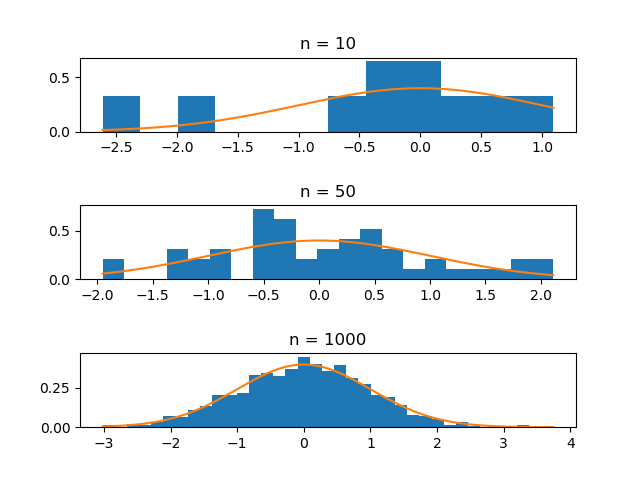
\includegraphics[width=0.8\textwidth]{1Normal.png}
  \caption{Нормальное распределение ~\eqref{eq:Normal}}
 
\end{figure}
\begin{figure}[H]
  \centering
  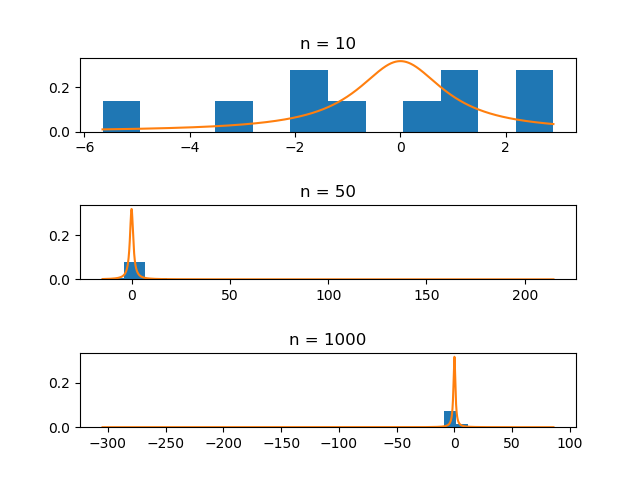
\includegraphics[width=0.8\textwidth]{1Cauchy.png}
  \caption{Распределение Коши ~\eqref{eq:Cauchy}}
\end{figure}
\begin{figure}[H]
\centering
  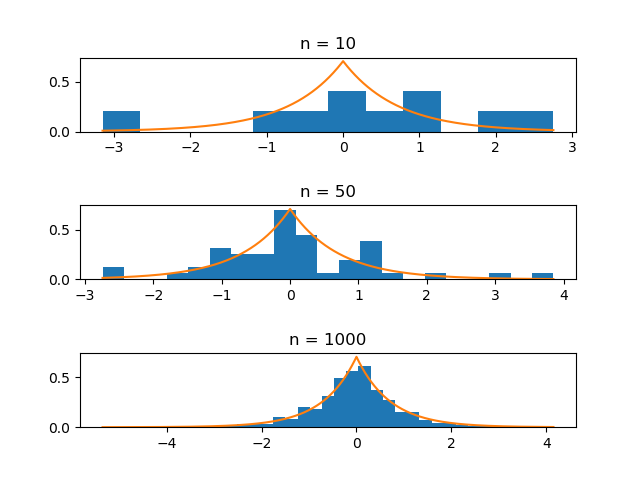
\includegraphics[width=0.8\textwidth]{1Laplace.png}
  \caption{Распределение Лапласа ~\eqref{eq:Laplace}}
\end{figure}
\begin{figure}[H]
  \centering
  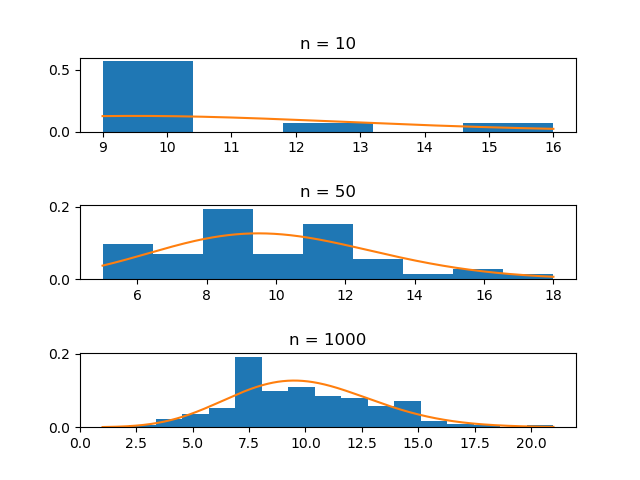
\includegraphics[width=0.8\textwidth]{1Poisson.png}
  \caption{Распределение Пуассона ~\eqref{eq:Poisson}}
\end{figure}
\begin{figure}[H]
  \centering
  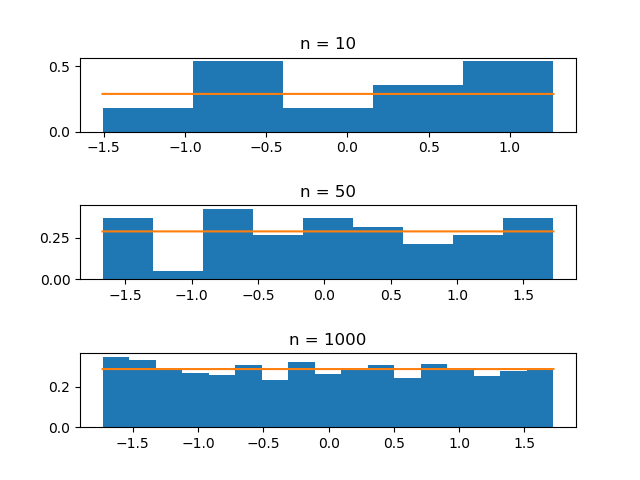
\includegraphics[width=0.8\textwidth]{1Uniform.png}
  \caption{Равномерное распределение ~\eqref{eq:Uniform}}
\end{figure}

\subsection{Таблицы значений}

\begin{table}[H]
  \centering
  \begin{tabular}{ | c | c | c | c | c | c | c | }
	\hline
	Normal n = 10 & & & & &  \\ \hline
	& $\overline x$~\eqref{eq:mean} & $med x$~\eqref{eq:mean}& $z_R $~\eqref{eq:semisum} & $z_Q $~\eqref{eq:semiquartile}  &  $z_{tr}$~\eqref{eq:trim}  \\ \hline
	$E(z) ~\eqref{eq:expectation}$ & -0.01 & 0.0 & 0.0 & 0.0 & -0.4 \\ \hline
	$D(z) ~\eqref{eq:dispertion}$ & 0.09935 & 0.13874 & 0.18181 & 0.11633 & 0.19166 \\ \hline
	
	Normal n = 100 & & & & &  \\ \hline
	& $\overline x$ & $med x$& $z_R $& $z_Q $&  $z_{tr}$\\ \hline
	$E(z)$ & 0.01 & -0.01 & 0.0 & 0.00 & -0.53 \\ \hline
	$D(z)$ & 0.05471 & 0.07758 & 0.13405 & 0.06471 & 0.11674 \\ \hline
	
	Normal n = 1000 & & & & &  \\ \hline
	& $\overline x$ & $med x$& $z_R $& $z_Q $&  $z_{tr}$\\ \hline
	$E(z)$ & 0.00 & -0.01 & 0.0 & 0.01 &-0.57 \\ \hline
	$D(z)$ & 0.03683 & 0.05231 & 0.11162 & 0.04357 & 0.08085 \\ \hline
	\end{tabular}
  \label{table:normal_table}
\caption{Нормальное распределение}
\end{table}


\begin{table}[H]
  \centering
  \begin{tabular}{ | c | c | c | c | c | c | c | }
	\hline
	Cauchy n = 10 & & & & &  \\ \hline
         & $\overline x$& $med x$& $z_R $ & $z_Q $  &  $z_{tr}$  \\ \hline
         $E(z)$ & 4 & 0 & 23 & 0 & -4 \\ \hline
         $D(z)$ & 15908.09147 & 0.43148 & 397531.77972 & 1.26249 & 523.04326 \\ \hline

Cauchy n = 100 & & & & &  \\ \hline
         & $\overline x$& $med x$& $z_R $ & $z_Q $  &  $z_{tr}$  \\ \hline
         $E(z)$ & 1 & 0.0 & -18 & 0.0 & -7 \\ \hline
         $D(z)$ & 8637.35792 & 0.22896 & 1880864.30928 & 0.65602 & 2509.25432 \\ \hline

Cauchy n = 1000 & & & & &  \\ \hline
         & $\overline x$& $med x$& $z_R $ & $z_Q $  &  $z_{tr}$  \\ \hline
         $E(z)$ & 1& 0.0 & 190 & 0.0 & -6 \\ \hline
         $D(z)$ & 6106.00336 & 0.15343 & 87773120.69259 & 0.43918 & 1712.09914 \\ \hline
	\end{tabular}
  \label{table:cauchy_table}
\caption{Распределение Коши}
\end{table}

\begin{table}[H]
  \centering
  \begin{tabular}{ | c | c | c | c | c | c | c | }
	\hline
Laplace n = 10 & & & & &  \\ \hline
         & $\overline x$& $med x$& $z_R $ & $z_Q $  &  $z_{tr}$  \\ \hline
         $E(z)$ & 0.0 & 0.00 & 0.0 & 0.0 & -0.4 \\ \hline
         $D(z)$ & 0.10735 & 0.08220 & 0.41080 & 0.11063 & 0.18386 \\ \hline

Laplace n = 100 & & & & &  \\ \hline
         & $\overline x$& $med x$& $z_R $ & $z_Q $  &  $z_{tr}$  \\ \hline
         $E(z)$ & 0.00 & 0.00 & 0.0 & 0.00 & -0.5 \\ \hline
         $D(z)$ & 0.05890 & 0.04395 & 0.40008 & 0.06062 & 0.11308 \\ \hline

Laplace n = 1000 & & & & &  \\ \hline
         & $\overline x$& $med x$& $z_R $ & $z_Q $  &  $z_{tr}$  \\ \hline
         $E(z)$ & 0.0 & 0.0 & 0.0 & 0.00 & -0.53 \\ \hline
         $D(z)$ & 0.03961 & 0.02948 & 0.40734 & 0.04075 & 0.07833 \\ \hline
	\end{tabular}
  \label{table:laplace_table}
\caption{Распределение Лапласа}
\end{table}

\begin{table}[H]
  \centering
  \begin{tabular}{ | c | c | c | c | c | c | c | }
	\hline
Poisson n = 10 & & & & &  \\ \hline
         & $\overline x$& $med x$& $z_R $ & $z_Q $  &  $z_{tr}$  \\ \hline
         $E(z)$ & 10.0 & 10 & 10 & 10 & 12 \\ \hline
         $D(z)$ & 0.94092 & 1.30249 & 1.90001 & 1.19398 & 1.61149 \\ \hline

Poisson n = 100 & & & & &  \\ \hline
         & $\overline x$& $med x$& $z_R $ & $z_Q $  &  $z_{tr}$  \\ \hline
         $E(z)$ & 10.0 & 9.9 & 11 & 10.0 & 12 \\ \hline
         $D(z)$ & 0.51966 & 0.74990 & 1.51329 & 0.67369 & 1.14114 \\ \hline

Poisson n = 1000 & & & & &  \\ \hline
         & $\overline x$& $med x$& $z_R $ & $z_Q $  &  $z_{tr}$  \\ \hline
         $E(z)$ & 10.0 & 9.9 & 11 & 10.0 & 12.6 \\ \hline
         $D(z)$ & 0.34978 & 0.50642 & 1.43907 & 0.45051 & 0.81966 \\ \hline
	\end{tabular}
  \label{table:poisson_table}
\caption{Распределение Пуассона}
\end{table}

\begin{table}[H]
  \centering
  \begin{tabular}{ | c | c | c | c | c | c | c | }
	\hline
Uniform n = 10 & & & & &  \\ \hline
         & $\overline x$& $med x$& $z_R $ & $z_Q $  &  $z_{tr}$  \\ \hline
         $E(z)$ & 0.0 & 0.0 & 0.01 & 0.0 & -0.4 \\ \hline
         $D(z)$ & 0.10099 & 0.23114 & 0.04599 & 0.13631 & 0.22124 \\ \hline

Uniform n = 100 & & & & &  \\ \hline
         & $\overline x$& $med x$& $z_R $ & $z_Q $  &  $z_{tr}$  \\ \hline
         $E(z)$ & 0.00 & 0.0 & 0.00 & 0.01 & -0.5 \\ \hline
         $D(z)$ & 0.05538 & 0.13012 & 0.02329 & 0.07517 & 0.13984 \\ \hline

Uniform n = 1000 & & & & &  \\ \hline
         & $\overline x$& $med x$& $z_R $ & $z_Q $  &  $z_{tr}$  \\ \hline
         $E(z)$ & 0.00 & 0.00 & 0.00 & 0.01 & -0.57 \\ \hline
         $D(z)$ & 0.03726 & 0.08778 & 0.01553 & 0.05062 & 0.09711 \\ \hline
	\end{tabular}
  \label{table:uniform_table}
\caption{Равномерное распределение}
\end{table}

\subsection{Упорядоченные характеристики положения}
\begin{enumerate}
\item Нормальное распределение:
\begin{equation}
\centering
z_{tr} \textless med \, x \textless \overline x= z_R \textless z_Q
\end{equation}

\item Распределение Коши:
\begin{equation}
\centering
z_{tr} \textless med \, x \textless \overline x = z_Q \textless z_R
\end{equation}

\item Распределение Лапласа:
\begin{equation}
\centering
z_{tr} \textless \overline x = med \, x = z_R = z_Q
\end{equation}

\item Распределение Пуассона:
\begin{equation}
\centering
med \, x \textless \overline x = z_Q \textless z_R \textless z_{tr}
\end{equation}

\item Равномерное распределение:
\begin{equation}
\centering
z_{tr} \textless \overline x = med \, x = z_R \textless z_Q
\end{equation}
\end{enumerate}

\subsection{Боксплот Тьюки}
\begin{figure}[H]
  \centering
  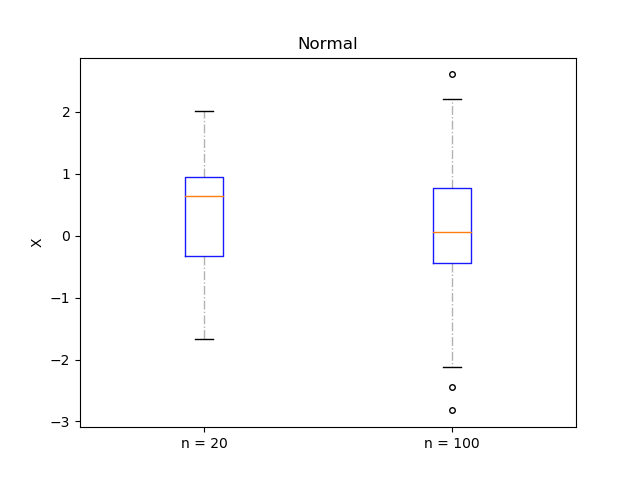
\includegraphics[width=0.8\textwidth]{3Normal.png}
  \caption{Нормальное распределение ~\eqref{eq:Normal}}
 
\end{figure}
\begin{figure}[H]
  \centering
  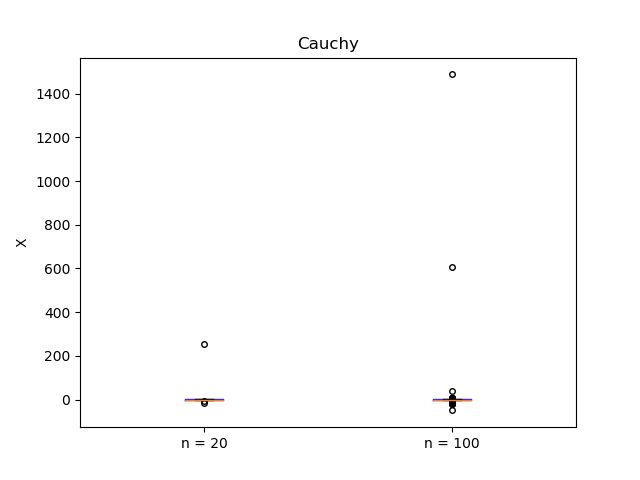
\includegraphics[width=0.8\textwidth]{3Cauchy.png}
  \caption{Распределение Коши ~\eqref{eq:Cauchy}}
\end{figure}
\begin{figure}[H]
\centering
  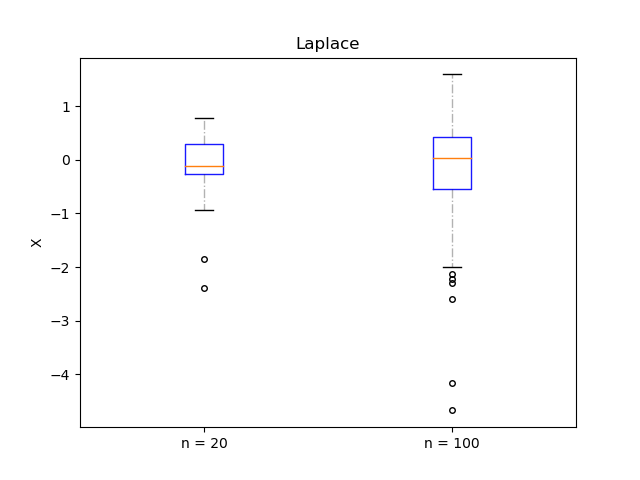
\includegraphics[width=0.8\textwidth]{3Laplace.png}
  \caption{Распределение Лапласа ~\eqref{eq:Laplace}}
\end{figure}
\begin{figure}[H]
  \centering
  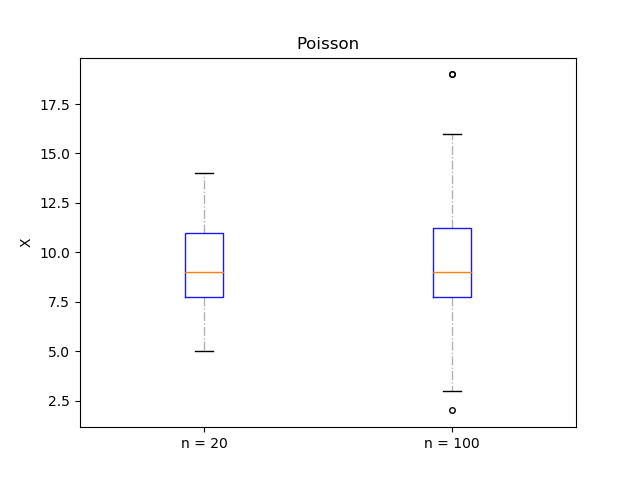
\includegraphics[width=0.8\textwidth]{3Poisson.png}
  \caption{Распределение Пуассона ~\eqref{eq:Poisson}}
\end{figure}
\begin{figure}[H]
  \centering
  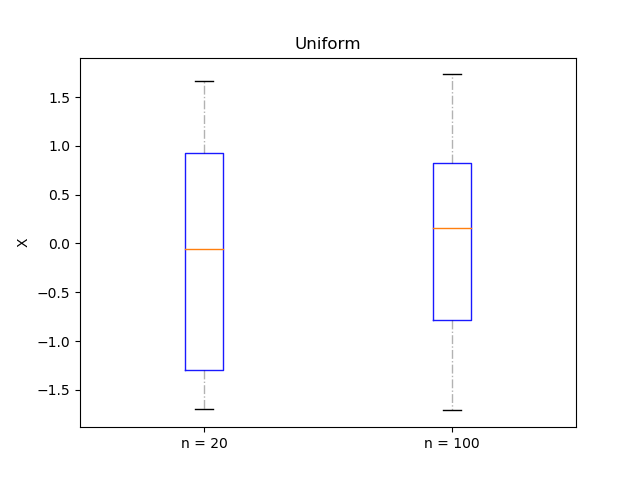
\includegraphics[width=0.8\textwidth]{3Uniform.png}
  \caption{Равномерное распределение ~\eqref{eq:Uniform}}
\end{figure}

\subsection{Доля выбросов}

\begin{table}[H]
  \centering
\begin{tabular}{| c | c | c |}
\hline
 Выборка  &   Среднее  & Дисперсия \\
\hline
 Normal, n = 20      &   0.017  & 0.001 \\
\hline
 Normal, n = 100     &  0.0095 & 0.0001 \\
\hline
 Cauchy, n = 20      &  0.139 & 0.005\\
\hline
 Cauchy, n = 100     &  0.154 & 0.001\\
\hline
 Laplace, n = 20     &  0.065 & 0.004\\
\hline
 Laplace, n = 100    & 0.0642 & 0.0009 \\
\hline
 Poisson, n = 20     &  0.016 & 0.002\\
\hline
 Poisson, n = 100    &  0.0101 & 0.0003\\
\hline
 Uniform, n = 20     & 0 & 0 \\
\hline
 Uniform, n = 100    &  0 & 0 \\
\hline
\end{tabular}
  \label{table:EjectionsProportion}
\caption{Доля выбросов}
\end{table}

\subsection{Теоретическая вероятность выбросов}

\begin{table}[H]
  \centering
\begin{tabular}{| c | c | c | c | c | c |}
\hline
Распределение  & $Q_1^T$ & $Q_3^T$ & $X_1^T$ & $X_2^T$ & $P_B^T$~\eqref{eq:prob1}~\eqref{eq:prob2}\\
\hline
Нормальное распределение & -0.674 & 0.674 & -2.698 & 2.698 & 0.007 \\
\hline
Распределение Коши & -1  & 1 & -4 & 4 & 0.156 \\
\hline
Распределение Лапласа & -0.490 & 0.490 & -1.961 & 1.961 & 0.063 \\
\hline
Распределение Пуассона & 8 & 12 & 2 & 18 & 0.008 \\
\hline
Равномерное распределение & -0.866 & 0.866 & -3.464 & 3.464 & 0 \\
\hline
\end{tabular}
  \label{table:TeorProb}
\caption{Теоретическая вероятность выбросов}
\end{table}

\subsection{Эмпирическая функция распределения}
\begin{figure}[H]
  \centering
  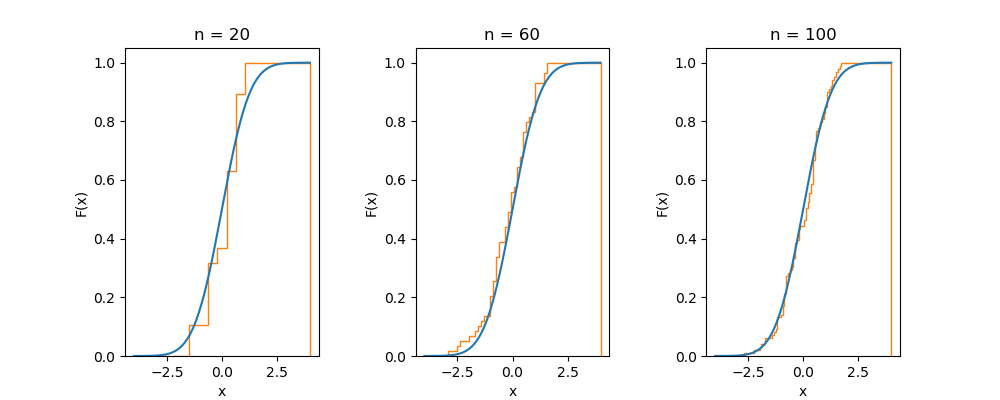
\includegraphics[width=1\textwidth]{4Normal.png}
  \caption{Нормальное распределение ~\eqref{eq:Normal}}
 
\end{figure}
\begin{figure}[H]
  \centering
  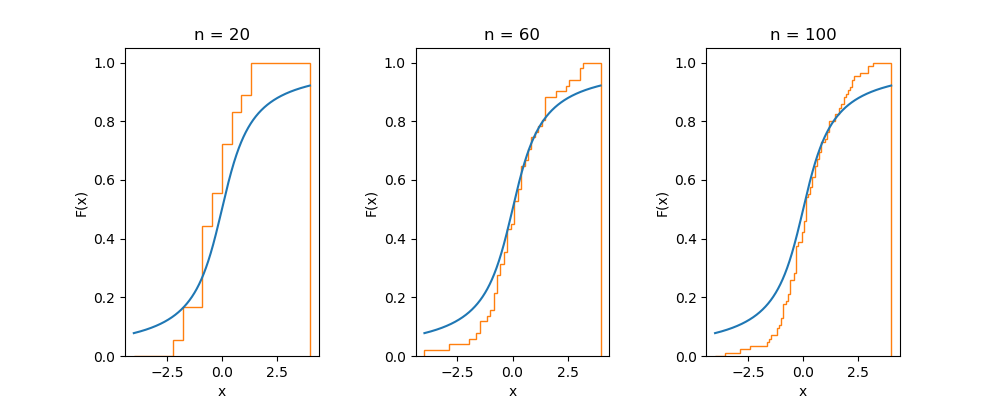
\includegraphics[width=1\textwidth]{4Cauchy.png}
  \caption{Распределение Коши ~\eqref{eq:Cauchy}}
\end{figure}
\begin{figure}[H]
\centering
  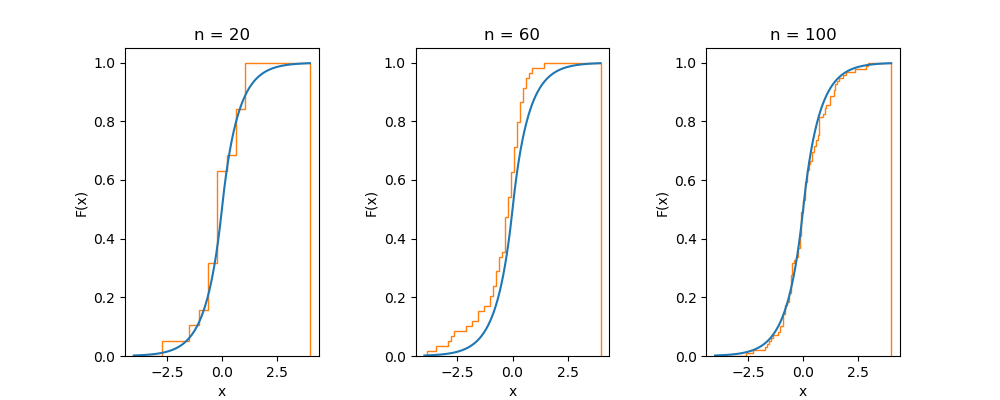
\includegraphics[width=1\textwidth]{4Laplace.png}
  \caption{Распределение Лапласа ~\eqref{eq:Laplace}}
\end{figure}
\begin{figure}[H]
  \centering
  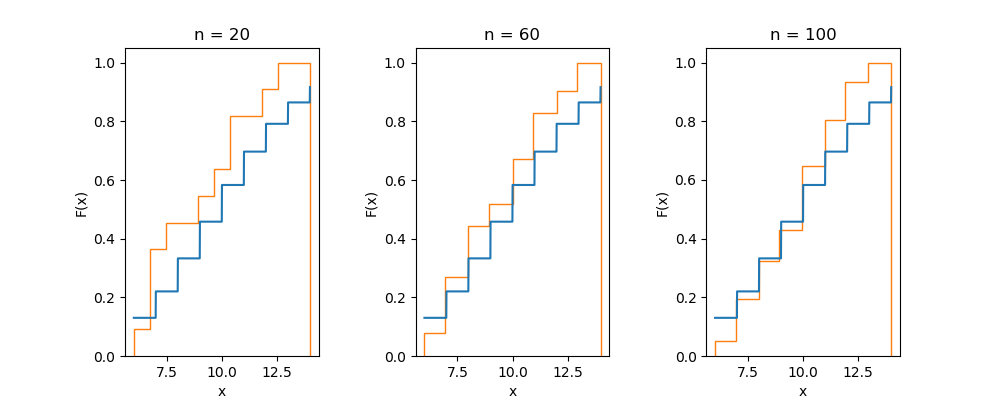
\includegraphics[width=1\textwidth]{4Poisson.png}
  \caption{Распределение Пуассона ~\eqref{eq:Poisson}}
\end{figure}
\begin{figure}[H]
  \centering
  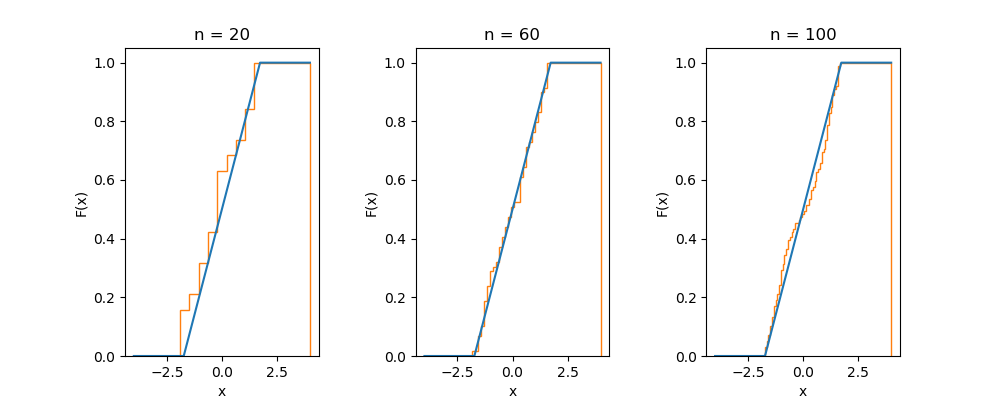
\includegraphics[width=1\textwidth]{4Uniform.png}
  \caption{Равномерное распределение ~\eqref{eq:Uniform}}
\end{figure}

\subsection{Ядерные оценки плотности распределения}
\begin{figure}[H]
  \centering
  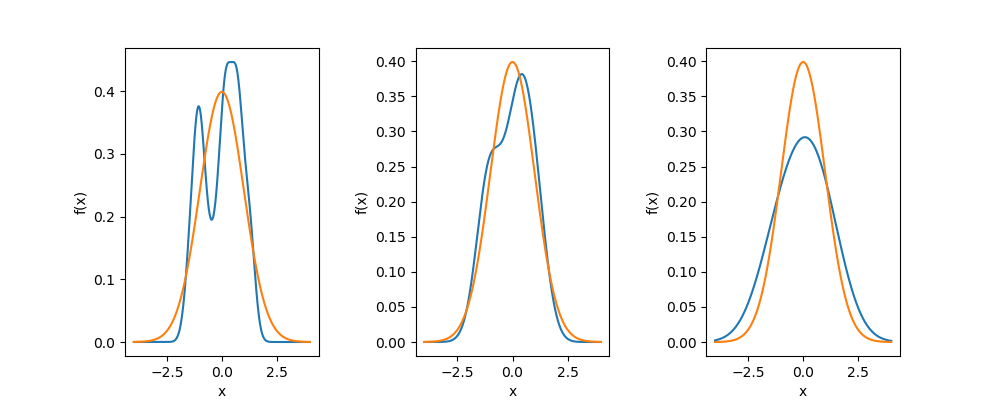
\includegraphics[width=1\textwidth]{Normalkernel20.png}
  \caption{Нормальное распределение, n = 20 ~\eqref{eq:Normal}}
\end{figure}

\begin{figure}[H]
  \centering
  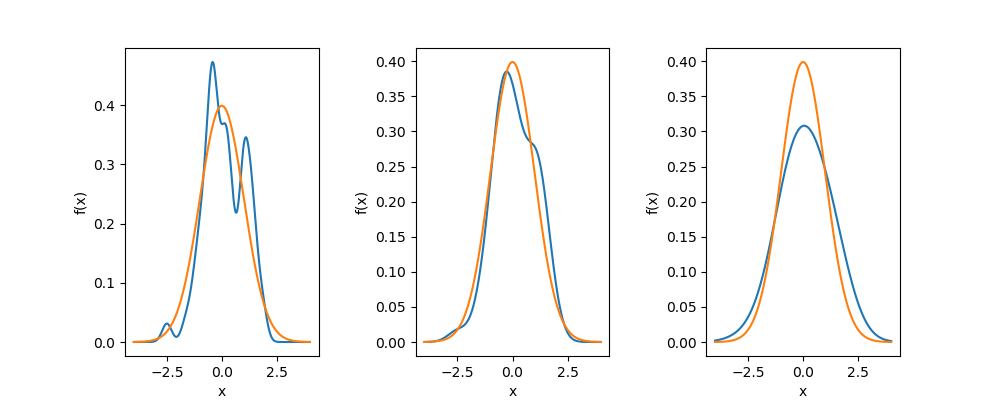
\includegraphics[width=1\textwidth]{Normalkernel60.png}
  \caption{Нормальное распределение, n = 60}
\end{figure}

\begin{figure}[H]
  \centering
  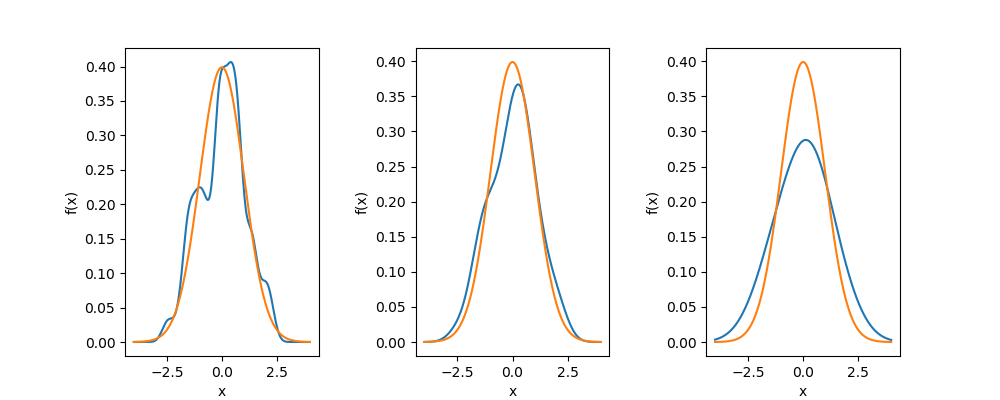
\includegraphics[width=1\textwidth]{Normalkernel100.png}
  \caption{Нормальное распределение, n = 100}
\end{figure}

\begin{figure}[H]
  \centering
  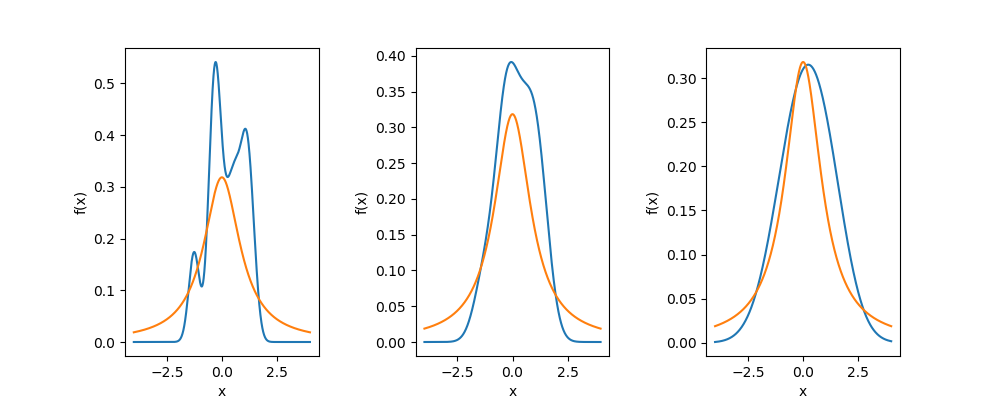
\includegraphics[width=1\textwidth]{Cauchykernel20.png}
  \caption{Распределение Коши, n = 20 ~\eqref{eq:Cauchy}}
\end{figure}

\begin{figure}[H]
  \centering
  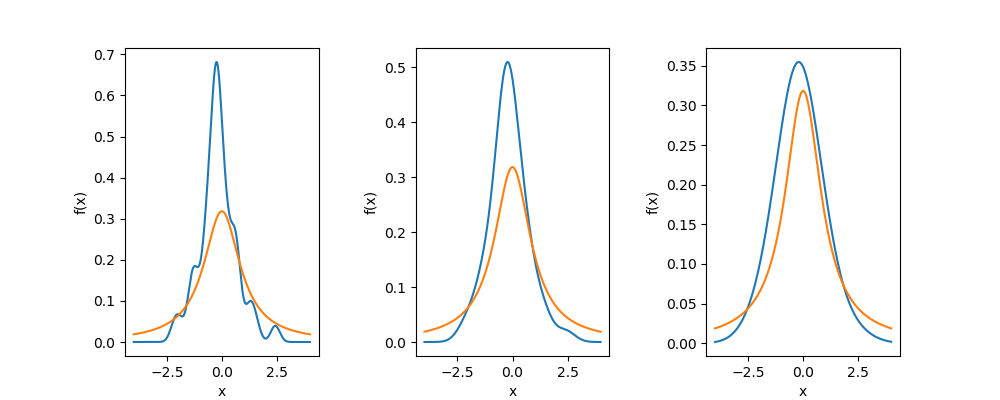
\includegraphics[width=1\textwidth]{Cauchykernel60.png}
  \caption{Распределение Коши, n = 60}
\end{figure}

\begin{figure}[H]
  \centering
  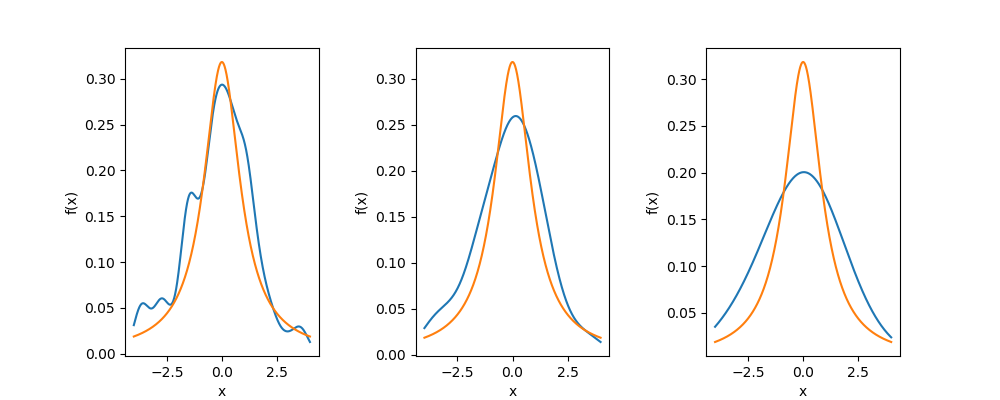
\includegraphics[width=1\textwidth]{Cauchykernel100.png}
  \caption{Распределение Коши, n = 100}
\end{figure}

\begin{figure}[H]
\centering
  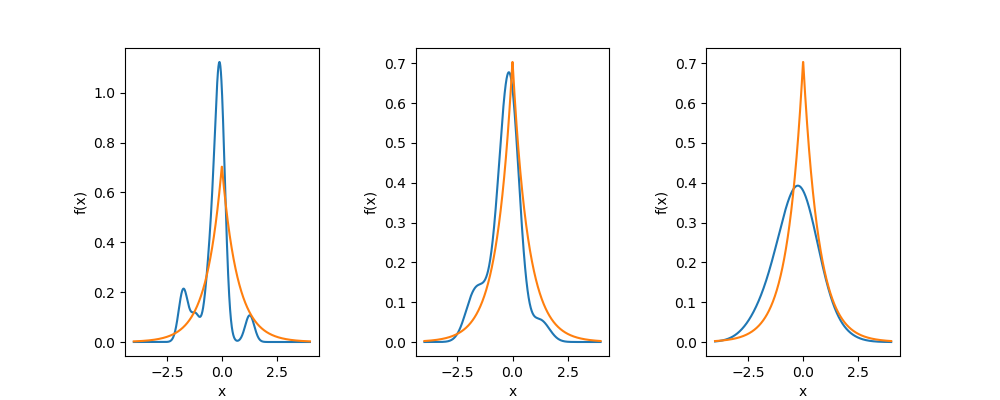
\includegraphics[width=1\textwidth]{Laplacekernel20.png}
  \caption{Распределение Лапласа, n = 20 ~\eqref{eq:Laplace}}
\end{figure}

\begin{figure}[H]
\centering
  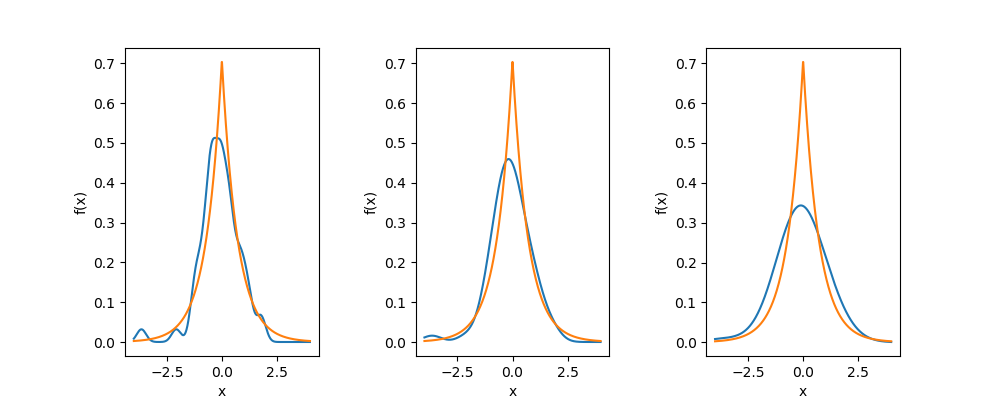
\includegraphics[width=1\textwidth]{Laplacekernel60.png}
  \caption{Распределение Лапласа, n = 60}
\end{figure}

\begin{figure}[H]
\centering
  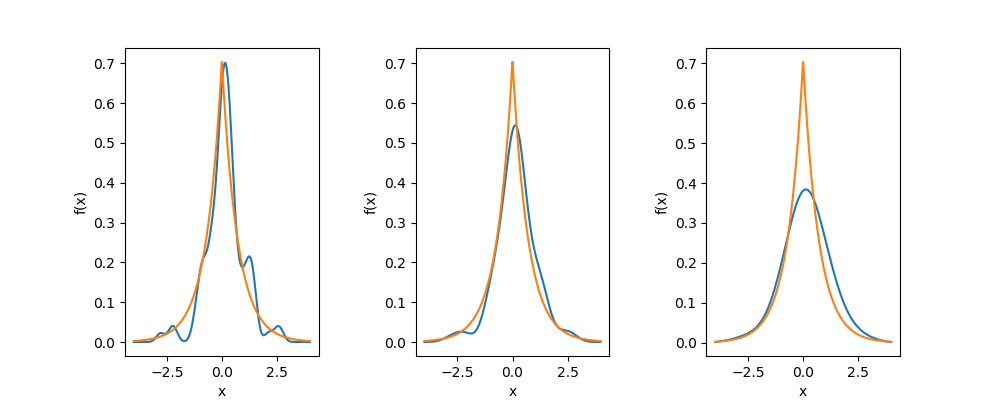
\includegraphics[width=1\textwidth]{Laplacekernel100.png}
  \caption{Распределение Лапласа, n = 100}
\end{figure}

\begin{figure}[H]
  \centering
  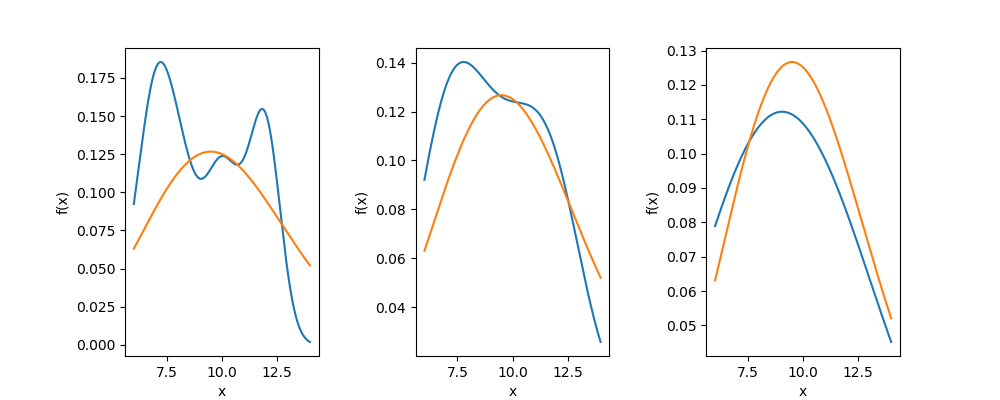
\includegraphics[width=1\textwidth]{Poissonkernel20.png}
  \caption{Распределение Пуассона, n = 20 ~\eqref{eq:Poisson}}
\end{figure}

\begin{figure}[H]
  \centering
  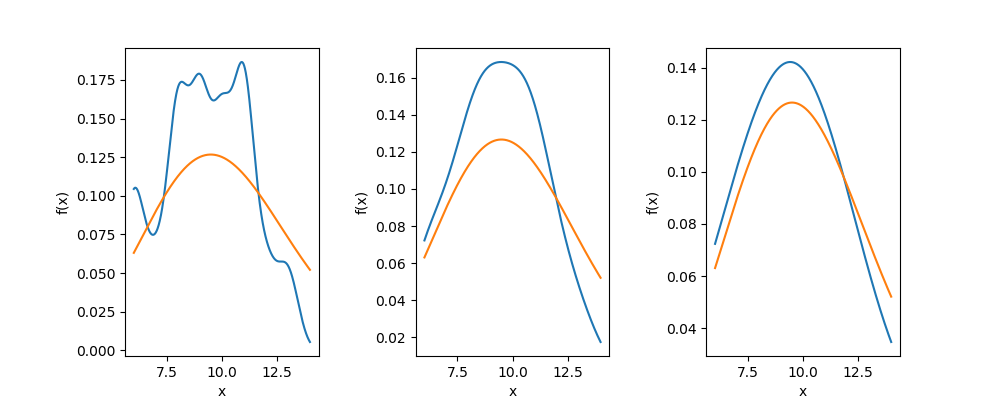
\includegraphics[width=1\textwidth]{Poissonkernel60.png}
  \caption{Распределение Пуассона, n = 60}
\end{figure}

\begin{figure}[H]
  \centering
  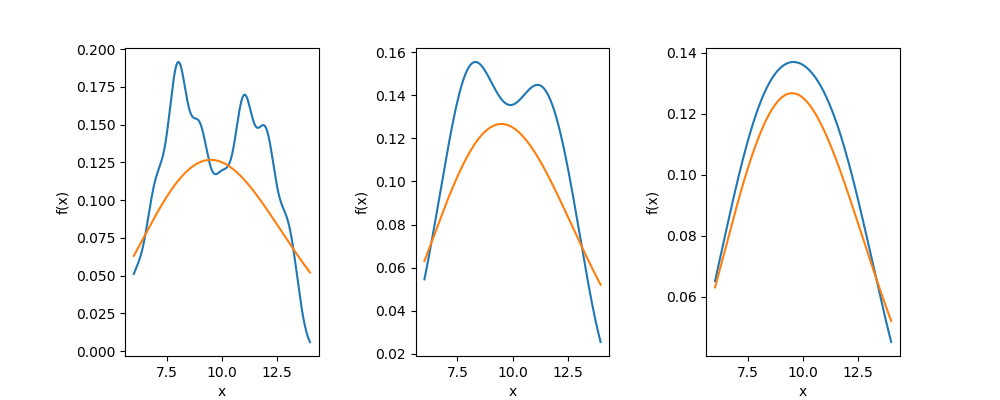
\includegraphics[width=1\textwidth]{Poissonkernel100.png}
  \caption{Распределение Пуассона, n = 100}
\end{figure}

\begin{figure}[H]
  \centering
  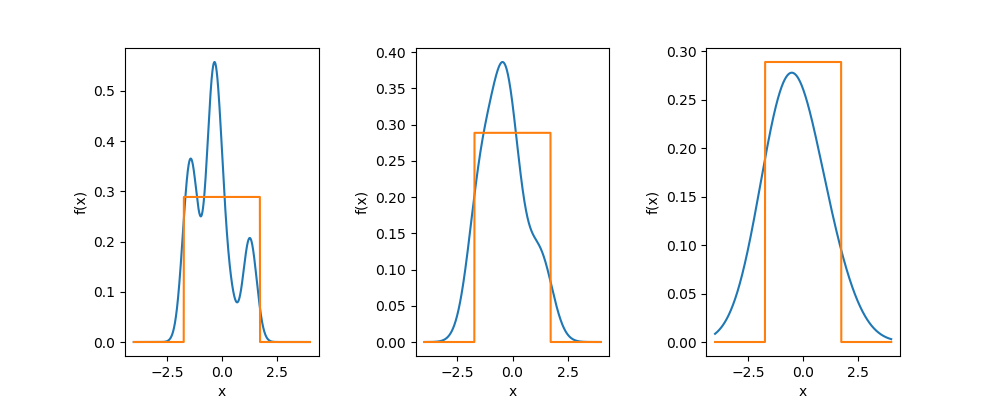
\includegraphics[width=1\textwidth]{Uniformkernel20.png}
  \caption{Равномерное распределение, n = 20 ~\eqref{eq:Uniform}}
\end{figure}

\begin{figure}[H]
  \centering
  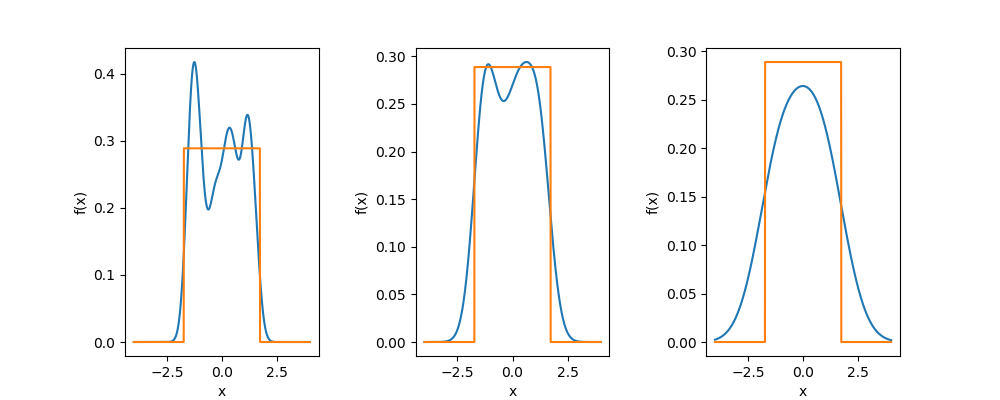
\includegraphics[width=1\textwidth]{Uniformkernel60.png}
  \caption{Равномерное распределение, n = 60}
\end{figure}

\begin{figure}[H]
  \centering
  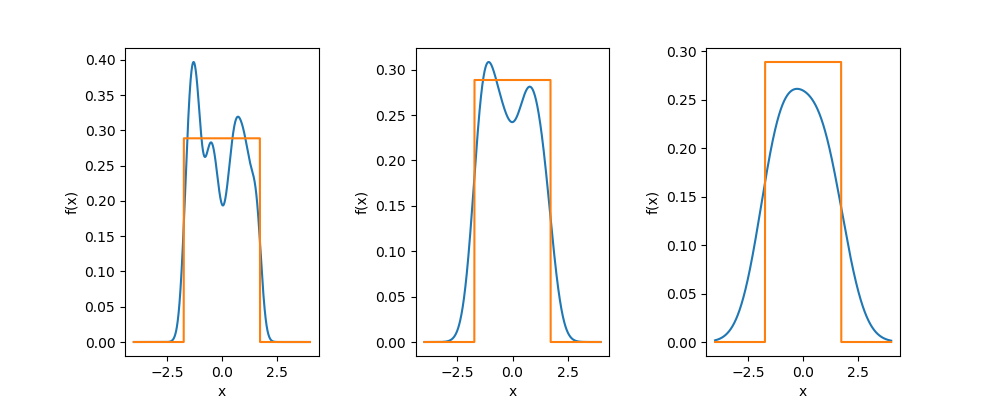
\includegraphics[width=1\textwidth]{Uniformkernel100.png}
  \caption{Равномерное распределение, n = 100}
\end{figure}


\section{Обсуждение}
\subsection{Гистограмма и график плотности распределения}

Из графиков видна чёткая зависимость, увеличение выборки увеличивает точность аппроксимации исходного распределения для всех распределений кроме Коши~\eqref{eq:Cauchy}.

\subsection{Характеристики положения и рассеяния}

Из полученных данных видно, что среднее~\eqref{eq:expectation} всех характеристик стремится к теоретическому, а оценка дисперсии~\eqref{eq:dispertion} к нулю при увеличении размера выборки. В случае распределения Коши~\eqref{eq:Cauchy} это верно только для медианы~\eqref{eq:med}.

\subsection{Доля и теоретическая вероятность выбросов}

Из полученных данных видно, что средняя доля выбросов (для 1000 эксперементов) стремится к теоретической оценке при увеличении размера выборки, для всех распределений, кроме распределения Пуассона~\eqref{eq:Poisson}. Дисперсия в свою очередь стремится к нулю уже для всех распределений. Также можно заметить, что для равномерного распределения отсутвуют выбросы, а вероятность их появления равна 0.

\subsection{Эмпирическая функция и ядерные оценки плотности распределения}

Из полученных данных видно, что точность аппроксимации эмпирической функцией~\eqref{eq:EmpDistr} распределения увеличивается с увеличением выборки. Для распределения Пуассона~\eqref{eq:Poisson} точность аппроксимации наименьшая. При увеличении размера выборки увеличевается точность аппроксимации плотности распределения для всех распределений кроме распределения Пуассона. Для нормального и равномерного распределения и рапределения Лапласа лучше подходит параметр $h = h_n$. Для рапределения коши и Пуассона лучше подходит параметр $h = \frac{h_n}{2}$

\section{Приложения}
Репозиторий на GitHub с релизацией: \href{https://github.com/WiillyWonka/MatStat}{github.com}.
\end{document}
